\documentclass[12pt]{article}
\usepackage[margin=1in]{geometry}
\usepackage[ampersand]{easylist}
\usepackage{tikz}
\usepackage{listings}
\usepackage{float}
\usepackage{fp}
\usepackage{amsmath,esint}
\usepackage{amssymb}
\usepackage{mathtools}
\usepackage{fancyhdr}
\usepackage[version=3]{mhchem}
\usepackage{textcomp}
\usepackage{mathtools}
\usepackage{circuitikz}
\usepackage{pgfplots}
\usepackage{titlesec}
\usepackage{amsfonts}
\usepackage{mathtools}
\usepackage{hyperref}
\usepackage{mathdots}
\usepackage{amsmath}

\hypersetup
{
  colorlinks,
  citecolor=black,
  filecolor=black,
  linkcolor=black,
  urlcolor=black
}
\pagestyle{fancy}

\rfoot{Page \thepage}
\rhead{}
\lhead{ECE337 Project Proposal Document}

\renewcommand{\headrulewidth}{0.4pt}

\titleformat*{\section}{\fontsize{16pt}{14pt}\selectfont\bfseries}

\usetikzlibrary{decorations.markings,patterns}
\usetikzlibrary{arrows}

\title{\vspace{-50pt}\textbf{\fontsize{14pt}{14pt}\selectfont Handwritten Digit Recognizer using a Neural Network}\vspace{-50pt}}
%\author{\textbf{Team Members:}\\ David Pimley, Dustin Andree,\\ Vadim Nikiforov, Chan Weng Yan}
\author{}
\date{}


\setlength\parindent{0pt}
\renewcommand{\L}{\mathcal L}
\newcommand{\Li}{\mathcal L^{-1}}
\renewcommand{\r}{\textrm}
\newcommand{\ra}{\rightarrow}
\newcommand{\lra}{\leftrightarrow}
\renewcommand{\a}{\forall}
\newcommand{\e}{\exists}
\newcommand{\bb}{\mathbb}
\renewcommand{\ss}{\subseteq}
\DeclarePairedDelimiter{\ceil}{\lceil}{\rceil}

\begin{document}

\maketitle
\section*{Team Members:}
{\fontsize{14pt}{14pt}\selectfont{\bf David Pimley:} \emph{David Pimley}\\[10pt]
{\bf Dustin Andree:} \emph{Dustin Andree}\\[10pt]
{\bf Vadim Nikiforov:} \emph{Vadim Nikiforov}\\[10pt]
{\bf Chan Weng Yan:} \emph{Chan Weng Yan}}
\section{Description and Rationale}
This project idea is a digit recognizer. It is designed to work with images consistent with the MNIST dataset, so it accepts 28$\times$28 px.~grayscale images, and outputs a detected digit. It accepts an image, and a list of weights and biases for the network connections. While it doesn't have an internal method for training, it outputs a cost function for each set of images, allowing for it to be connected to an external training module. Furthermore, using SPI, the network model can be reprogrammed on the fly. Digit recognition is a very useful application, as it allows for devices to interpret data ranging from checks to signs to handwritten notes. Machine learning allows for very high accuracy for digit detection, and when applied to digit recognition can handle a wide range of fonts and handwriting styles. However, due to the structure of neural networks, sequential computation such as what is found in microcontrollers is not effective for a neural network. Instead, devices such as GPUs are often used due to their capacity for parallel computation. This device uses an architecture specialized just for multiplying weights and adding inputs, allowing for much faster computation for digit recognition. While on a microcontroller this system would require tens of thousands of sequential multiplications, on an ASIC this device will have critical paths with only 3-4 multiplications necessary before the output. This is done by taking advantage of the \texttt{MapReduce} procedure, where in this case the mapping is applying weights to the biases, and the reduction is adding together all the inputs to a sigmoid, and then calculating the sigmoid output (which can be done by a lookup table.) Finally, this device allows for training to be done on separate hardware, which typically requires far more computational power than detection, and then allows the trained model to be uploaded on the fly using a standard interface (In this case, SPI) allowing for flexible operation.
\newpage

\section{Design Architecture}
\begin{figure}[H]
  \centering
  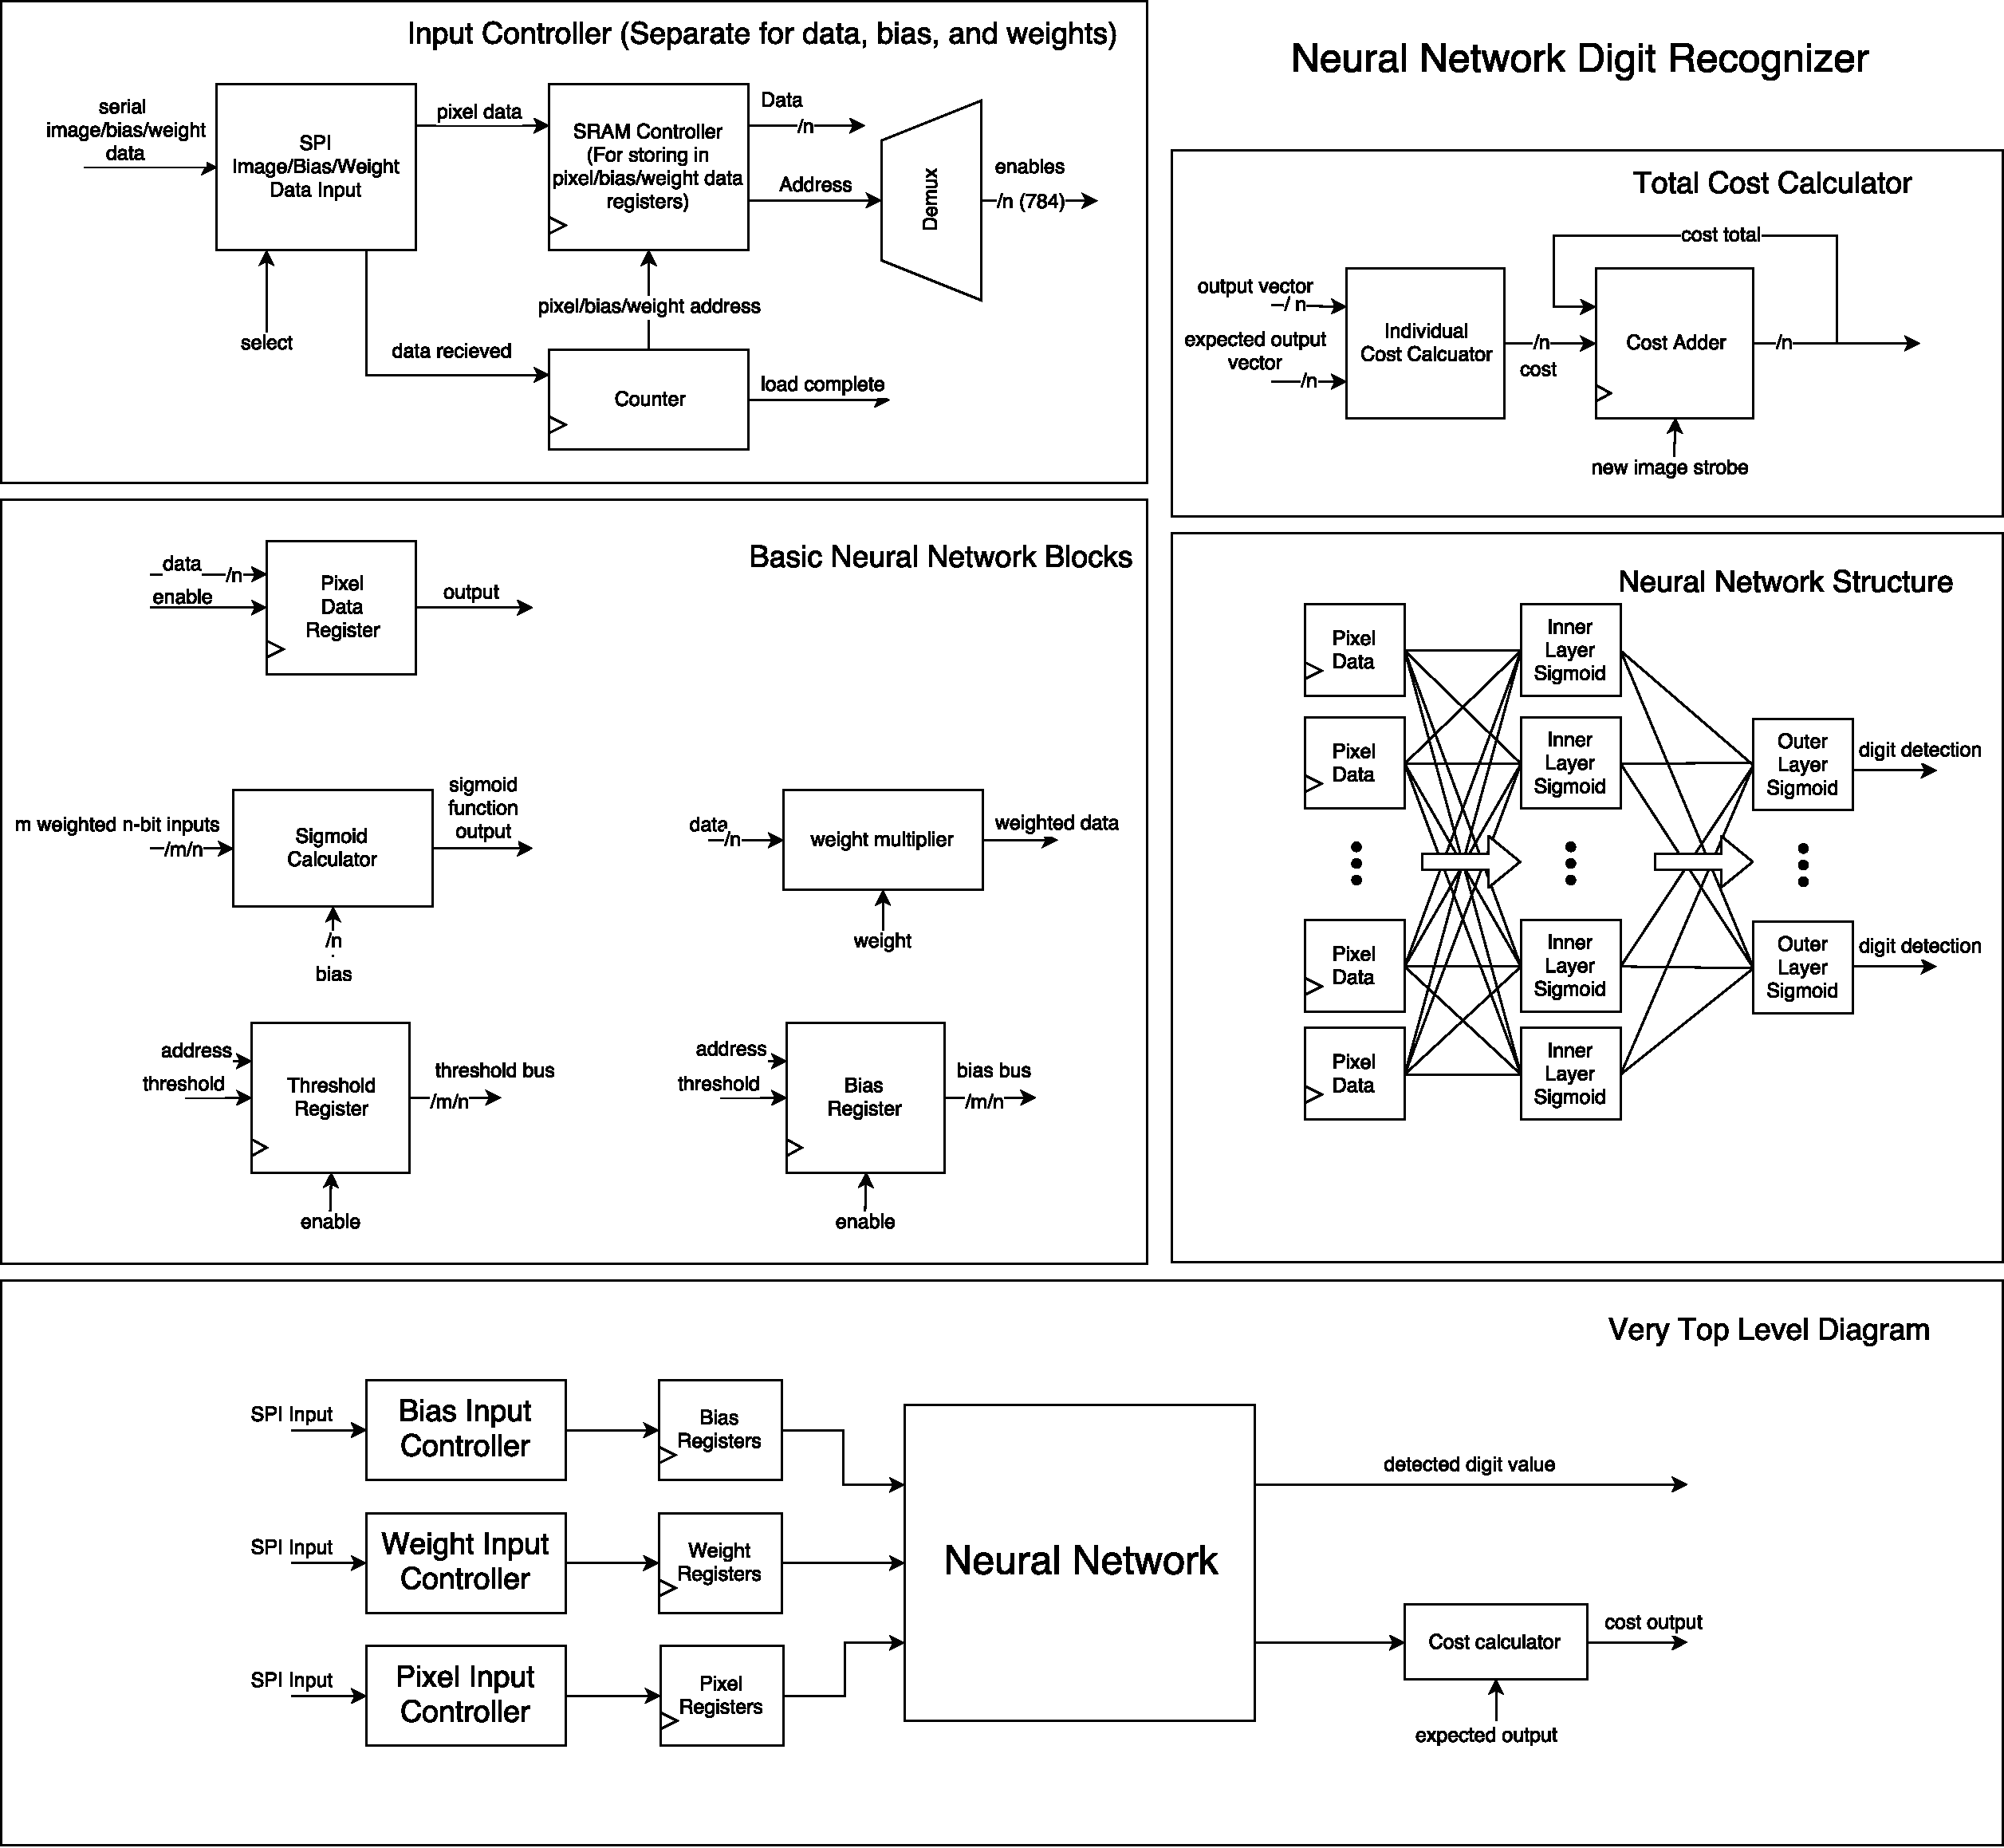
\includegraphics[width=\textwidth]{digit_recognizer.pdf}
\end{figure}

\end{document} 


